% !TeX root = ../economia.tex
\chapter{Domanda}
Dal punto di vista dell’impresa, \`e fondamentale comprendere le scelte di acquisto dei
\gls{consumatori} in relazione al bene o servizio offerto (\emph{domanda}) e il comportamento delle altre imprese
presenti sul mercato (\emph{concorrenza}).
Così come le imprese mirano a massimizzare il profitto, i consumatori acquistano e consumano beni o
servizi per aumentare il proprio benessere o \gls{utilita}.

\section{Funzione di utilità}

I consumatori massimizzano la funzione di utilità tenendo in considerazione i propri vincoli di bilancio
(la spesa per l’acquisto di beni non può essere superiore al reddito)

\paragraph{Utilità monotona e crescente}
il consumo di un determinato bene fa aumentare l’utilità del
consumatore.

\paragraph{Utilità marginale decrescente}
l’utilità addizionale (marginale) di ogni successiva unità di consumo è
sempre minore.

\section{Prezzo di riserva (PR)}

Il \emph{prezzo di riserva} è il prezzo massimo che un consumatore è disposto a pagare per acquistare
un’unità di un bene.

Consumatori diversi hanno prezzi di riserva diversi per lo stesso bene e non hanno incentivi a rivelare il proprio prezzo di riserva alle imprese produttrici.

\begin{itemize}
	\item PR > Prezzo praticato da imprese produttrici $\rightarrow$ Acquisto
	\item PR < Prezzo praticato da imprese produttrici $\rightarrow$ Non acquisto
\end{itemize}

\section{Curva di domanda}
La \emph{curva di domanda individuale} di un bene $x$ esprime, per ciascun consumatore, il \emph{prezzo di riserva} di
diverse quantità di $x$. La curva di domanda individuale indica
all’impresa che produce $x$ quante unità
acquista il consumatore dato un prezzo.
\begin{center}
	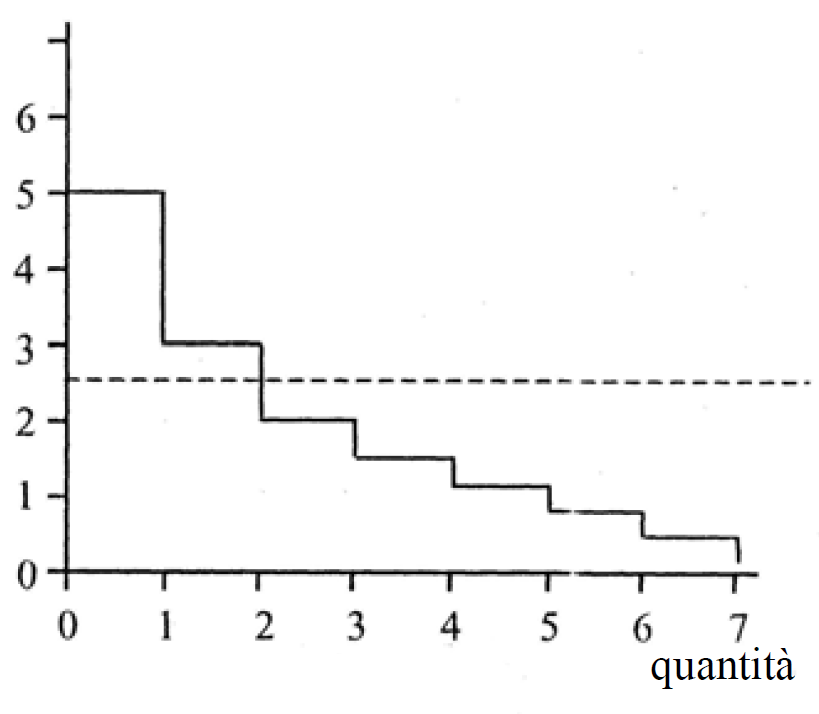
\includegraphics[width=0.3\linewidth]{images/curva_di_domanda}
\end{center}

La curva di domanda individuale è decrescente:
\begin{itemize}
	\item Prezzo $\uparrow \quad$ Domanda $\downarrow$
	\item Prezzo $\downarrow \quad$ Domanda $\uparrow$
\end{itemize}

Il prezzo di riserva è legato all’utilità marginale:
\begin{itemize}
	\item dipende dalla quantità del bene già consumata
	\item la variazione di utilità in seguito all’acquisto e consumo di un’unità aggiuntiva del bene (utilità
	marginale) è decrescente
\end{itemize}

La curva di domanda individuale consente di valutare il \emph{surplus del consumatore}, cioè la differenza fra il
prezzo che un consumatore è disposto a pagare e il prezzo di mercato del bene.

\section{Determinanti della domanda individuale}
\subsection{Caratteristiche del consumatore}
\begin{enumerate}
	\item Gusti e necessità (preferenze) del consumatore
	\begin{itemize}
		\item Esempio: la quantità di Coca Cola domandata da un individuo dipende al fatto che la Coca Cola gli piaccia o meno (\emph{gusti}) e dalla sua sete (\emph{necessità})
	\end{itemize}
	\item Reddito o ricchezza del consumatore
	\begin{itemize}
		\item \emph{Beni normali}: la quantità domandata aumenta all’aumentare del reddito
		\item \emph{Beni inferiori}: la quantità domandata diminuisce all’aumentare del reddito
	\end{itemize}
\end{enumerate}

\subsection{Caratteristiche del bene}
\begin{enumerate}
	\item Prezzo e disponibilità di \emph{beni sostituti}, cioè beni che espletano funzioni simili a quelle del bene in oggetto $x$. Se aumenta (diminuisce) il prezzo di un sostituto di $x$, la quantità domandata di $x$ aumenta
	(diminuisce).
	\item Prezzo e disponibilità di \emph{beni complementari}, cioè beni che tendono a essere consumati insieme a $x$. Se aumenta (diminuisce) il prezzo di un bene complementare a $x$, la quantità domandata di $x$
	diminuisce (aumenta).
\end{enumerate}

\section{Domanda di Mercato}
La \emph{domanda di mercato} è la somma, per tutti gli $N$ consumatori, delle quantità
domandate individuali:
\[
Q(p) = \sum^N_{i=1} q_i(p)
\]

\section{Elasticità della domanda} 

L'\emph{elasticità della domanda} è la variazione della quantità domandata al variare di una delle sue componenti:
\begin{itemize}
	\item Prezzo del bene
	\item Prezzo degli altri beni
	\item Reddito del consumatore
\end{itemize}

Una misurazione accurata della variazione della domanda al variare delle sue componenti consente di
conoscere le reazioni dei consumatori e quindi l’impatto che tali variazioni hanno sui ricavi dell’impresa.

\paragraph{Elasticità della domanda al prezzo} variazione percentuale della quantità domandata del bene $x$ a
seguito della variazione percentuale del suo prezzo.

\[
\sigma_x = \left| \frac{\delta q_x}{\delta p_x} \frac{p_x}{q_x} \right| 
\]

L’elasticità della domanda rispetto al prezzo dipende non solo dalla pendenza costante della curva
di domanda, ma anche dal prezzo e dalla quantità.

La domanda di un bene con pochi sostituti è poco elastica (anelastica), cioè ha una curva più ripida.

\subsection{Elasticità incrociata}
L'elasticità incrociata del bene $x$ rispetto a $y$ è la variazione percentuale della quantità domandata del bene $x$ a
seguito della variazione percentuale del prezzo del bene $y$.
\[
\sigma_{xy} = \frac{\delta q_x}{\delta p_y} \frac{p_y}{q_x}
\]

Il segno dipende dalle relazioni di complementarietà e sostituibilità tra i beni:
\begin{itemize}
	\item \emph{Beni complementari}: elasticità incrociata negativa
	\item \emph{Beni sostituti}: elasticità incrociata positiva
\end{itemize}

\subsection{Elasticità al reddito}
L'elasticità al reddito del bene $x$ è la variazione percentuale della quantità domandata del bene $x$ a seguito della
variazione percentuale del reddito $M$.

\[
\sigma_{M} = \frac{\delta q_x}{\delta M} \frac{M}{q_x}
\]

Il segno dipende dalla natura del bene:
\begin{itemize}
	\item \emph{Beni normali}: elasticità della domanda al reddito positiva
	\item \emph{Beni inferiori}: elasticità della domanda al reddito negativa
\end{itemize}

Un bene di prima necessità avrà $\sigma_M < 1$, mentre un bene di lusso avrà $\sigma_M > 1$.